\documentclass{article}
\usepackage{amsmath}
\usepackage{array}
\usepackage{color}
\usepackage{graphicx}
\usepackage{float} %utiliser H pour forcer a mettre l'image ou on veut
\usepackage{lscape} %utilisation du mode paysage
\usepackage{mathbbol} % permet d'avoir le vrai symbol pour les reels grace a mathbb
\usepackage{enumerate}
\usepackage{marvosym}
\usepackage{moreverb} % permet d'utiliser verbatimtab : conservation la tabulation
\usepackage{url}
\usepackage{stmaryrd} % permet d'utiliser \llbracket et \rrbracket : double crochet


\setlength {\textwidth}{16cm}
\setlength {\textheight}{21cm}
\setlength {\oddsidemargin}{0cm}
\setlength{\headsep}{5pt} 

\newcommand\bn{\boldsymbol{\nabla}}
\newcommand\bo{\boldsymbol{\Omega}}
\newcommand\br{\mathbf{r}}
\newcommand\la{\left\langle}
\newcommand\ra{\right\rangle}
\newcommand\bs{\boldsymbol}
\newcommand\red{\textcolor{red}}
\newcommand\pk{\partial K}
\newcommand\ldb{\{\!\{}
\newcommand\rdb{\}\!\}}
\newcommand\llb{\llbracket}
\newcommand\rrb{\rrbracket}

\renewcommand{\(}{\left(}
\renewcommand{\)}{\right)}
\renewcommand{\[}{\left[}
\renewcommand{\]}{\right]}


\begin{document}
\title{Coupled Electron-Photon Transport\\
\small{Dissertation Proposal}}
\author{Bruno Turcksin, Department of Nuclear Engineering} 
\date{}
\maketitle

% Introduction
\section{Introduction}


% Current state of the problem
\section{Current state of the problem}
There are two parts of the problem. First, we need to solve the transport
equation for the photons and the electrons and then, we need to solve the
optimization problem.
\subsection{Transport equation for the photons and the electrons}
The equation that we want to solve is the Boltzmann-CSD equation (the
variables are omitted for \hbox{brevity) :}
\begin{equation}
\begin{split}
\bo \cdot \bn \Psi + \Sigma_t \Psi = \int_{4\pi}\int_0^{\infty}
\Sigma_s\(\bo\cdot\bo', E'\rightarrow E\)\Psi\(\bo',E'\)dE' d\bo'+
\frac{\partial S \Psi}{\partial E} +Q
\label{b-csd}
\end{split}
\end{equation}
where :
\begin{itemize}
\item $\Psi$ is the angular flux
\item $\Sigma_t$ is the smooth-component of the total macroscopic cross
section
\item $\Sigma_s$ is the smooth-component of the macroscopic differential
scattering cross section
\item $Q$ is a volumetric source
\item $\bo = (\mu,\phi)$
\item $\mu$ is the cosine of the directional polar angle
\item $\phi$ is the directional azimuthal angle
\item $S$ is the restricted stopping power :
\begin{equation}
S(E) = 2\pi \int_0^E \int_{-1}^1 \Sigma_{ss} (E\rightarrow E',\mu_0)
\(E-E'\)d\mu_0 dE'
\end{equation}
\item $\mu_0 = \mu' \mu + \sqrt{\(1-\mu'^2\)\(1-\mu^2\)} \cos\(\phi'-\phi\)$
\item $\Sigma_{ss}\(E\rightarrow E', \mu_0\)$ denotes the forward-peaked
scattering cross section.
\end{itemize}
Standard boundary conditions can be applied to (\ref{b-csd}), the most likely
being the vacuum boundary conditions :
\begin{equation}
\Psi(\br,\bo,E) = 0\ \textrm{ for } \bo \cdot \bs{n} < 0 \ \textrm { and } \br
\in \partial \mathcal{D}_v
\end{equation}
and the incoming flux boundary conditions :
\begin{equation}
\Psi(\br,\bo,E) = g(\br,\bo,E)\ \textrm{ for } \bo \cdot \bs{n} < 0 \ \textrm { and } \br \in \partial \mathcal{D}_i
\end{equation}
where $\partial \mathcal{D}_v$ is the boundary of the domain where vacuum
conditions are applied and $\partial \mathcal{D}_i$ is the boundary of the
domain where incoming flux conditions are applied.\\
The state-of-art for deterministic electron-photon calculation is the code
Acuros\cite{acuros}. It employs linear discontinuous finite-element on
unstructured mesh consisting of tetrahedral elements and an adaptive mesh
refinement method. It uses a discrete ordinates for the angular discretization 
and compute the first
collision source by computing an analytical uncollided flux. The
energy discretization is done with standard multigroup method and the
energy derivative of the CSD operator is discretized using linear
discontinuous finite-element.

\subsection{Optimization problem}
The modern radiotherapy uses the Intensity Modulated Radiation Therapy (IMRT) as 
one of the methods to treat cancer. IMRT allows several beams with 
different intensity profiles and the goal is to deliver a sufficient dose to the 
tumor while sparing healthy organs. To optimize the intensity profile, it is very 
common to divide the beams in small beamlets, each of them having a constant 
intensity. In a real application, the number of beamlets is around a thousand. 

This problem is very complex and a lot of objective functions and constraints 
\cite{math,complexity,minima,dose-volume} have been 
proposed. Moreover, there are a lot of methods \cite{dose-volume} used to solve 
these optimization problems such as Monte-Carlo method with steepest descent
\cite{complexity}, linear programming, filtered back-projection, simulated
annealing, dynamically penalized likelihood, projections onto convex, active
set method and simulated dynamics\cite{dose-volume}.

The most used objective function is :
\begin{equation}
\min  \sum_{(i,j,k)\in \mathcal{T}} \(D_{ijk}-\delta_{ijk}\)^2 
\label{objective}
\end{equation}
where $\delta_{ij}$ is the prescribed dose for the voxel $ijk$, $D_{ijk}$ is the
actual dose for the voxel and $\mathcal{T}$ is the tumor. 

This objective function tries to to minimize the difference between the planned 
dose and the dose in the tumor. The constraints used are dose-volume constraints
\cite{complexity,minima,dose-volume}. The idea is that we do not want to have more 
than a given percentage of the volume of an organ to receive more than a given dose. 
Mathematically, we have for each constraint :
\begin{equation} 
\sum_{ijk \in \mathcal{D}} \nu\(D_{ijk}-\delta_{ijk}\)\frac{V_{ijk}}{V} \leq \gamma
\label{constraint}
\end{equation}
where $V_{ij}$ is the volume of voxel $ij$, $V$ is the total volume of the organ, 
$\nu(x)$ is the Heaviside function, $\gamma$ is the tolerance percentage
volume and $\mathcal{D}$ is the domain studied. We also impose the dose to be 
positive or zero :
\begin{equation}
D_{ij} \geq 0
\label{constraint2}
\end{equation}

It is well known that even if the objective function is convex, the problem has 
several local minima \cite{minima}. The reason is that because the domain is not 
convex, the number of local minima can increase factorially with the number of 
beamlets. Since we can have more than a thousand beamlets, the 
number of local minima can be large. To avoid the local minima problem, 
we can rewrite the optimization problem as a mixed-integer linear problem. 
This does not have local minima but the calculation time can be prohibitive 
\cite{minima}.  



% Proposed research
\section{Proposed research}
The proposed research seeks to be able to compute the optimized position
and intensity of the photon beams as fast as possible. To do that, we need to
develop on three different topics :
\begin{itemize}
\item massive parallelization
\item efficient and fast algorithms to solve the transport problem
\item optimization of the intensity of the beams 
\end{itemize}

\subsection{Massive parallelization}
Parallelization is an important way to decrease the time needed to solve the
transport and the optimization problem. To do this, we will use
the capabilities of the Parallel Deterministic Transport code developed at
Texas A\&M University. 

\subsection{Efficient and fast algorithms}
This section consists in mainly three parts. The first one is the energy
discretization. We plan to use linear discontinuous finite element for the
energy discretization. This discretization scheme has shown good behavior
(less oscillations than the diamond difference scheme) for the self-adjoint
angular flux form of the equation (\ref{b-csd}) \cite{saaf} and the 
Boltzmann-Fokker-Planck equation \cite{fem}.\\
We need to define : 
\begin{align}
& \Delta E^g = E^{g-1/2} -E^{g+1/2}\\
& E^g = \frac{E^{g-1/2}+E^{g+1/2}}{2}\\
& \Psi^g(\br) = \int_{\Delta E^g} dE \Psi(\br,E)\\
& \Psi(\br,E) = \Psi^{g,T}\cdot b^g \ \ \forall E \in \[E^{g+1/2},E^{g-1/2}\]\\
& \Psi^g =
\begin{pmatrix}
\Psi_x^g\\
\Psi_E^g
\end{pmatrix}
\ \ \forall E \in \[E^{g+1/2},E^{g-1/2}\]\\
& b^g = 
\begin{pmatrix}
b_{\br}^g(\br,E)\\
b_E^g(E)
\end{pmatrix}
\ \ \forall E \in \[E^{g+1/2},E^{g-1/2}\]\\
& b_{\br}^g\(x,E\) = \frac{b_{\br}(\br)}{\Delta E^g}\ \ \forall \in
\[E^{g+1/2},E^{g-1/2}\]\\
& b_{\br} \textrm{ are discontinuous finite element basis functions}\\
& b_E^g\(E\) = \frac{2}{\(\Delta E^g\)^2} \(E-E^g\)\ \ \forall \in
\[E^{g+1/2},E^{g-1/2}\]\\
&\lim_{E\underset{>}{\to}E^{g+1/2}} E = E^{g+1/2,+}\\
&\lim_{E\underset{>}{\to}E^{g-1/2}} E = E^{g-1/2,+}\\
& K \textrm{ is a cell}
\end{align}  
Using this energy discretization and upwind in energy, (\ref{b-csd}) becomes :
\begin{equation}
\begin{split}
&\Delta E^g \oint_{\pk} \(\bo \cdot \bs{n}\) \Psi_{\br}^{g} \(b_{\br}^g(\br,E^g) 
\cdot b_{\br}^{g,T}(\br,E^g)\) ds - \Delta E^g \int_K \(\Psi_{\br}^{g,T} \cdot 
b_{\br}^g\(\br,E^g\)\) \(\bo_d \cdot \bn b_{\br}^{g}\(\br,E^g\)\) d\br\\
&+ \Delta E^g \int_K \Sigma_t^g\(\br\) \Psi_{\br}^{g}\(b_{\br}^{g}(\br,E^g)\cdot 
b_{\br}^{g,T}\(\br,E^g\)\) d\br = \int_k \sum_{g'=1}^G \sum_{l=0}^L \sum_{m=-l}^l 
\Delta E^{g'} \frac{2l+1}{4\pi} \Sigma_{s,l}^{g'\rightarrow g}(\br)\\
&\Phi_{l}^{m,g'} Y_m^l\(\bo_d\)\(b_{\br}^{g',T}(r,E^{g'})\cdot b_{\br}^g\(\br,E^g\)\) 
d\br + \int_{K} d\br \(S^{g-1}(\br)\(\Psi^{g-1,T}\cdot b^{g-1}\(\br,E^{g-1/2,+}\)\)
\right.\\
& - S^{g}(\br) \left. \(\Psi^{g,T}\cdot b^g\(\br,E^{g+1/2,+}\)\)\) b_{\br}^g
(\br,E^g)
\end{split}                                   
\end{equation}          
\begin{equation}
\begin{split}
&\frac{\Psi_E^g}{3\Delta E^g} \int_K \Sigma_t(d\br) d\br =
\sum_{l=0}^L \frac{2l+1}{4\pi} \sum_{m=l}^l \frac{\Phi_l^{m,g}
Y_l^m\(\bo_d\)}{3} \int_K \Sigma_{s,l}^{g' \rightarrow g}\(\br\) d\br \\
&\int_K \frac{S^{g-1}(\br)}{\Delta E^g} \(\Psi_d^{g-1,T}(\br) \cdot
b^{g-1}(\br,E^{g-1/2})\) d\br - \int_K \frac{S^g}{\Delta E^g} \(\Psi_d^{g,T}
\cdot b_{\br}^g (\br,E^{g+1/2}) +\Psi_E^g\) 
\end{split}
\end{equation}   
The second part is to implement an efficient preconditioner. The most 
common method to accelerate the convergence of the transport equation is to use 
a P1 Synthetic Acceleration scheme (P1SA) or a Diffusion Acceleration scheme 
(DSA) \cite{adams}. Next we present the P1SA equation but first let us write the primal and the adjoint angular fluxes as :
\begin{align}
& \Psi_m = \frac{1}{4 \pi} \left(\Phi + 3 \boldsymbol{J}\cdot
\boldsymbol{\Omega}_m\right) \label{eq1}\\
& \Psi_m^* = \frac{1}{4 \pi} \left(\Phi + 3 \boldsymbol{J}^*\cdot
\boldsymbol{\Omega}_m\right) \label{eq2}
\end{align}
The $S_N$ variational form of the transport equation for neutral particle is given 
by (see also \cite{jcam}) :
\begin{equation}
b(\Psi,\Psi^*) - \sum_{e\in\partial \mathcal{D}^r} \sum_{\boldsymbol{\Omega}_m \cdot \boldsymbol{n}_b < 0} w_m \left\langle\Psi_{m'},\Psi_m^*\right\rangle_e - \sum_{n=0}^N \sum_{k=-n}^n \frac{2n+1}{4\pi} \left(\Sigma_{s,n}\Phi_{n,k},\Phi_{n,k}^*\right)_{\mathcal{D}} = l(\Psi^*)
\end{equation}
where the bilinear and the linear forms are :
\begin{equation}
\begin{split}
b(\Psi,\Psi^*) &= \sum_{d=1}^M w_m \left(\left(\boldsymbol{\Omega}_m \cdot \boldsymbol{\nabla}+\Sigma_t\right)\Psi_d,\Psi_d^*\right)_{\mathcal{D}} + \sum_{d=1}^M \left\langle\llbracket\Psi_d\rrbracket,\Psi_d^{*+}\right\rangle_{E_h^i}\\
&+\sum_{e\in\partial \mathcal{D}} \sum_{\boldsymbol{\Omega}_d \cdot \boldsymbol{n}_b < 0} w_d \left\langle\Psi_d,\Psi_d^*\right\rangle_e
\end{split}
\end{equation}
\begin{equation}
l(\Psi^*) = \sum_{l=0}^L \sum_{m=-l}^l
\left(Q_{l,m},\Phi_{l,m}^*\right)_{\mathcal{D}} + \sum_{e\in\partial
\mathcal{D}^d} \sum_{\bo_d \cdot \boldsymbol{n}_b} w_d
\left\langle\Psi_d^{inc},\Psi_d^*\right\rangle_e
\end{equation}
where :
\begin{itemize}
\item $\mathcal{D}$  is the domain. 
\item $\partial\mathcal{D}$ is the boundary of the domain.
\item $\partial\mathcal{D}^r$ is the reflective boundary of the domain.
\item $\partial\mathcal{D}^d$ is the Dirichlet boundary of the domain.
\item $\boldsymbol{n}_b$ is the normal vector on the domain boundary.
\item $\Psi_d^{\pm} = \lim_{s\to 0^{\pm}} \Psi_d (\boldsymbol{r} + s \boldsymbol{\Omega}_d)$
\item $\llbracket\Psi_d\rrbracket = \Psi_d^+ - \Psi_d^-$ is the inter element jump.
\item $E_h^i$ is the set of all interior edges.
\item $(f,g)_{\mathcal{D}} = \sum_{K \in \mathcal{T}} (f,g)_K$ with  $(f,g)_K = \int_K f\ g\ d\mathbf{r}$
\item $\left\langle f,g\right\rangle_{\mathcal{D}} = \sum_{e \in \mathcal{E}_h^i} \left\langle f,g\right\rangle_e$ with  $\left\langle f,g\right\rangle_e = \int_e \left| \boldsymbol{\Omega}_m \cdot \boldsymbol{n}(\mathbf{r})\right| ds$
\item $Q_{l,m}$ are the moments volumetric source (scattering and fixed external source).
\end{itemize}
Using (\ref{eq1}) and (\ref{eq2}) in the bilinear and  linear form, we find
after some algebra :
\begin{equation}
b\left(\Phi,\boldsymbol{J},\Phi^*,\boldsymbol{J}^*\right) = l\left(\Phi^*,\boldsymbol{J}^*\right)
\label{P1SA}
\end{equation}
with :
\begin{equation}
\begin{split}
b(\Phi,\boldsymbol{J},\Phi^*,\boldsymbol{J}^*) &= \left(\Sigma_a \Phi,\Phi^*\right)_D + \left(3\Sigma_{tr} \boldsymbol{J},\boldsymbol{J}^*\right)_D+\left(\boldsymbol{\nabla} \Phi,\boldsymbol{J}^*\right)_D - \left(\boldsymbol{J},\boldsymbol{\nabla} \Phi^*\right)_D\\
&+ \frac{1}{4} \left(\llbracket\Phi\rrbracket,\llbracket\Phi^*\rrbracket\right)_{E_h^i}+\left(\llbracket\Phi\rrbracket,\ldb\boldsymbol{J}^*\rdb\cdot\boldsymbol{n}\right)_{E_h^i} -
\left(\ldb\boldsymbol{J}\cdot\boldsymbol{n}\rdb,\llbracket\Phi^*\rrbracket\right)_{E_h^i}\\
& + \frac{9}{16}\left(\llbracket \boldsymbol{J}\cdot\boldsymbol{n}\rrbracket,\llbracket \boldsymbol{J}^*\cdot\boldsymbol{n}\rrbracket\right)_{E_h^i} + \frac{9}{16}\left(\llbracket\boldsymbol{J}\rrbracket, \llbracket \boldsymbol{J}^*\rrbracket\right)_{E_h^i}\\
&+\frac{1}{4}\left(\Phi,\Phi^*\right)_{\partial D^d} + \frac{1}{2} \left(\Phi,\boldsymbol{J}\cdot \boldsymbol{n}\right)_{\partial D^d} - \frac{1}{2}\left(\boldsymbol{J}\cdot\boldsymbol{n},\Phi^*\right)_{\partial D^d}\\
&+\frac{9}{16}\left(\boldsymbol{J},\boldsymbol{J}^*\right)_{\partial D^d} + \frac{9}{16}\left(\boldsymbol{J}\cdot\boldsymbol{n},\boldsymbol{J}^*\cdot\boldsymbol{n}\right)_{\partial D^d}+\frac{9}{4} \left(\boldsymbol{J}\cdot\boldsymbol{n}, \boldsymbol{J}\cdot\boldsymbol{n}\right)_{\partial D^r}
\end{split}
\end{equation}
and :
\begin{equation}
l(\Phi^*,\boldsymbol{J}^*) = \left(Q_0,\Phi^*\right)_D + \left(3\boldsymbol{Q}_1,\boldsymbol{J}^*\right)_D + \left(J^{inc},\Phi^*\right)_{\partial D^d} - \left(\boldsymbol{\Upsilon}^{inc},\boldsymbol{J}^*\right)_{\partial D^d}
\end{equation}
where $Q_0$ is the zeroth moment of the source, $\boldsymbol{Q}_1$ is the first moment of the source :
\begin{equation}
J^{inc} = -\sum_{\boldsymbol{\Omega}_d \cdot \boldsymbol{n}(\boldsymbol{r}_b)<0} w_d |\boldsymbol{\Omega}_d \cdot \boldsymbol{n}\left(\boldsymbol{r}_b)\right)| \Psi_d^{inc}
\end{equation}
$\Phi^d$ is the flux on the Dirichlet boundary and :
\begin{equation}
\boldsymbol{\Upsilon} = - \sum_{\boldsymbol{\Omega}_d \cdot \boldsymbol{n}(\boldsymbol{r}_b)<0} 3w_d\boldsymbol{\Omega}_d |\boldsymbol{\Omega}_d \cdot \boldsymbol{n}\left(\boldsymbol{r}_b)\right)| \Psi_d^{inc}
\end{equation}
The problem with the P1SA or the DSA methods is that they are not stable when the 
anisotropy is too large. The acceleration scheme that we presented converges for 
any anisotropy when the medium is thick but not when
the cells are thin. Since in (\ref{b-csd}) we approximate the 
forward-peaked scattering of the electrons by a Dirac distribution, the 
anisotropy is very large. Thus, we will have to modify the acceleration scheme 
used. We already studied some 
properties of this scheme when the updating method is modified \cite{russe} and 
when the number of sweeps, which use the acceleration scheme, has been modified
\cite{multisweep}. The results were encouraging but they have to be confirmed for
electron transport which is much more anisotropic that what we have tried. If
the acceleration scheme remains instable while using the previous methods,
generalisation of the Modified $P_N$ Synthetic Acceleration or the Modified
DSA \cite{kassem} will be used.\\
The last interesting algorithm is the algorithm to compute the uncollided flux 
in parallel. The standard algorithms to compute the uncollided flux are not 
scalable. They either require to have the whole mesh in memory or the processors 
close to the source do most of the work.\\ 
The first collision source can be easily expressed mathematically by rewriting 
(\ref{b-csd}) using operator notation :
\begin{align}
&L \Psi = H \Phi + Q\\
&\Psi = \Psi^{inc}
\end{align}

\begin{align}
&L \(\Psi^u + \Psi^c\) = H \(\Phi^u + \Phi^c\) + Q\\
&\Psi^u + \Psi^c = \Psi^{inc}
\end{align}
That we can rewrite :
\begin{align}
& L\Psi^u = 0\\
& \Psi^u = \Psi^{inc}
\end{align}

\begin{align}
& L\Psi^c = H \Phi^u + H\Phi^c + Q \label{last}\\
& \Psi^c = 0
\end{align}

If we have several groups, we can rewrite (\ref{last}) :
\begin{equation}
L \Psi^{c,g} = H \Phi^{c,g} + H \Phi ^{u,g} + \sum_{g'\neq g}H\Phi^{g'}+Q
\end{equation}

% Optimization part
\subsection{Optimization of the intensity of the beams}
\subsubsection{Preliminary results}
We have already tried several methods : active set method, penalty method
and simulated annealing.We used these methods with a  two dimensional code for 
neutral particles instead of the three dimensional photon-electron problem. 

\paragraph{Active method}
The first method we tried was a variant of the active set method inspired by
\cite{dose-volume}. The algorithm works as follow :
\begin{itemize}
\item Step 1 : Optimize the dose without any constraint.
\item Step 2 : Sort the voxel in the healthy organs by their received dose
from a low dose to a high dose.
\item Step 3 : Apply the constraint $D_{ijk}<\delta_{ijk}$ on the $(1-\gamma)
N$ voxels with the lowest dose ($N$ is the number of voxels for the organ) for
each organ,
\item Step 4 : Solve the constrained optimization problem using the active set
method.
\item Step 5 : Go back to Step 3 until the solution cannot be improved
anymore. 
\end{itemize}
This method is rapid but does not give reliable results when the solution of the
constrained problem is very different from the solution of the unconstrained
problem. 

\paragraph{Penalty method}
Instead of minimizing a constrained optimization problem, we solve an unconstrained problem :
\begin{equation}
\min Q_{\mu} (x) = f(x) + \frac{1}{2\mu} \|g(x)\|^2 + \frac{1}{2\mu} \|\[h(x)\]^-\|^2
\end{equation}
where :
\begin{equation}
\[h(x)\]^- = \min \{0,h(x)\}
\end{equation}
We decrease the value of the parameter $\mu$ during the optimization process.
We have the following objective function :
\begin{equation}
f = \sum_{(i,j)\in \mathcal T} \(D_{ijk} - \delta_{ijk}\)^2
\end{equation}
The constraints are given by :
\begin{align}
&h_1 = \gamma - \sum_{ijk \in \mathcal{D}} \frac{V_{ijk}}{V} \nu \(D_{ijk} -
\delta_{ijk}\) \geq 0 \label{dv}\\
&h_2 = D_{ijk} \geq 0
\end{align}
Thus, we have the following quadratic relaxation :
\begin{equation}
Q_{\mu} = \sum_{(i,j,k)\in \mathcal T} \(D_{ijk} - \delta_{ijk}\)^2 +
\frac{1}{2\mu} \(\[\gamma - \sum_{(i,j,k) \in \mathcal{D}} \frac{V_{ijk}}{V}
\nu \(D_{ijk} - \delta_{ijk}\)\]^-\)^2 + \frac{1}{2\mu} \(\[D_{ijk}\]^-\)^2
\end{equation}
If we want to use the steepest descent or Newton's method to solve the
previous problem, we need to take the derivative of the Heaviside function and
this is an issue because the derivative is a Dirac distribution. Therefore, 
we use the following \hbox{approximation :}
\begin{equation}
\nu (x) = \frac{1}{1+e^{-2\alpha x}}
\end{equation}
where $k$ is a large constant.
The gradient of the quadratic relaxation is :
\begin{equation}
\begin{split}
\bn Q_{\mu} &= \sum_{(i,j,k) \in \mathcal{T}} 2 \(D_{ijk} - \delta_{ijk}\) \bn
D_{ijk} + \frac{1}{\mu} \(\[\gamma - \sum_{(i,j,k) \in
\mathcal{D}}\frac{V_{ijk}}{V} \frac{1}{1+e^{-2k\(D_{ijk} - \delta_{ijk}\)}}\]^-\) \times\\
&\(\sum_{(i,j,k)\in \mathcal{D}}\frac{V_{ijk}}{V} \frac{-2\alpha
e^{-2\alpha\(D_{ijk}-\delta_{ijk}\)} \bn
D_{ijk}}{\(1+e^{-2\alpha(D_{ijk}-\delta_ijk)}\)^2}\)+ \frac{1}{\mu} \(\[D_{ijk}\]^-\)
\end{split}
\end{equation}
If we look at the second term of the previous equation, we see that the
penalty term disappear when the constraint is satisfied (like it should) but
also that the penalty term can be arbitrary close to zero by increasing the dose.
The problem is that the derivative of the logistic is very close to zero and
approaches zero when $x$ increases. Thus, by increasing the dose, we can
decrease that term faster than we decrease $\mu$.
We see that we need to modified the constraints if we want to use the penalty method. To do that, we replaced the Heaviside function $\nu(x)$ by the following function :
\begin{equation}
\tilde{\nu}(x) = \left\{
\begin{aligned}
&x & \textrm{if } x\geq 0\\
&0 & \textrm{else}
\end{aligned}
\right.
\end{equation}
Thus, (\ref{dv}) becomes :
\begin{align}
\widetilde{h}_1 = \gamma - \sum_{ijk\in\mathcal{D}} \frac{V_{ijk}}{V}
\frac{\tilde{\nu}\(D_{ijk}-\delta_{ijk}\)}{\delta_{ijk}} \geq 0
\end{align}
where we had to renormalize the new function to keep $\gamma$ adimensional. We have 
the new quadratic relaxation :
\begin{equation}
Q_{\mu} = \sum_{(i,j,k)\in \mathcal{T}} (D_{ijk}-\delta_{ijk})^2 +
\frac{1}{2\mu} \(\[\gamma - \sum_{(i,j,k) \in \mathcal{D}} \frac{V_{ijk}}{V}
\frac{\tilde{\nu} \(D_{ijk} - \delta_{ijk}\)}{\delta_{ijk}}\]^-\)^2 +
\frac{1}{2\mu} \(\[D_{ijk}\]^-\)^2
\end{equation}
The gradient of the constraint is given by :
\begin{equation}
\begin{split}
\bn Q_{\mu} &= \sum_{(i,j,k) \in \mathcal{T}} 2 \(D_{ijk} - \delta_{ijk}\) \bn
D_{ijk} + \frac{1}{\mu} \(\[\gamma-\sum_{(i,j,k)\in\mathcal{D}}
\frac{V_{ijk}}{V} \frac{\tilde{\nu}(D_{ijk}-\delta_{ijk})}{\delta_{ijk}}\]^-\) 
\times\\
&\sum_{(i,j,k)\in \mathcal{D}} \frac{V_{ijk}}{V} \frac{\[- \bn
D_{ijk}\]^-}{\delta_{ijk}}  + \frac{1}{\mu}\(\[D_{ijk}\]^-\)
\end{split} 
\end{equation}
The Hessian is given by : 
\begin{equation}
\begin{split}
\bn^2 Q_{\mu} &= \sum_{(i,j)\in \mathcal{T}} 2 \(\bn D_{ij}\) \cdot \(\bn D_{ij}\)^T + \frac{1}{\mu} \(\sum_{(i,j)\in \mathcal{D}} \frac{V_{ij}}{V} \frac{\[-\bn D_{ij}\]^-}{\delta_{ij}}\) \cdot \\
&\(\sum_{(i,j)\in \mathcal{D}} \frac{V_{ij}}{V} \frac{\[- \bn D_{ij}\]^-}{\delta_{ij}} \)^T + \frac{1}{\mu} \[I\]^-
\end{split}
\end{equation}
Because the penalty method start by solving an unconstrained problem and then
use the solution as the initial point for the constrained problem, the
results are very similar to the one of the previous method.

\paragraph{Simulated annealing}
We tried three different simulated annealing programs \cite{scipy,wagner,asamin}.
The simulated annealing of SciPy\cite{scipy} is the most efficient of the
three but, like the two others, it failed to produce an acceptable result for 
complicated cases. All three algorithms gave as result a local minima far away
from the global minimum.

\subsubsection{Future work}
We investigate other methods like the use of the HOPSPACK library \cite{hopspack}, 
which is a package using a derivative-free algorithm. At each iteration, 
the program generates a trial point along the positive and negative direction 
of each coordinate axis. The set of search directions are centered on the 
current best point and initially extend a certain fixed distance. If one 
of these trial points improves the objective function, then it becomes the 
new best point for the next iteration. If a trial point does worse, then the 
step size in that direction is reduced to generate a replacement trial point. 
The process ends when the step length becomes sufficiently short in every 
direction.\\
Another method that we might try is based on a Peano space-filling curve 
\cite{livre}. The idea is to reduce the problem to a H\"{o}lder one-dimensional 
one. Having a one dimensional problem, the core algorithm can be written as :
$x$ = input and $z$ = outcome, ($z=\phi(x)$)
\begin{itemize}
\item Step 1 : Renumber the points :
\begin{equation}
a=x_0 <x_1<\ldots<x_k=b
\end{equation}
\item Step 2 : Compute the maximal slope :
\begin{equation}
\begin{split}
M &= \max_{1\leq i\leq k} \left| \frac{z_i - z_{i-1}}{x_i -x_{i-1}} \right|\\
&= \max\(M_{k-1},\frac{|z_{k+1}-z_{t-1}|}{x_{k+1}-x_{t-1}},\frac{|z_{t}-z_{k+1}|}{x_{t}-x_{k+1}}\)
\end{split}
\end{equation}
\item Step 3 : Accept the estimate :
\begin{equation}
m =\left\{
\begin{aligned}
1, &\ M=0\\
rM, &\ M>0
\end{aligned}
\right.
\end{equation}
where $r>1$ is the input of the algorithm.\\
\item Step 4 : For each interval $(x_{i-1},x_i)$, $1\leq i \leq k$, calculate the value :
\begin{equation}
R(i) = m(x_i - x_{i-1}) + \frac{(z_i-z_{i-1})^2}{m(x_i-x_{i-1})}-2(z_i + z_{i-1})
\end{equation}
called characteristic of the interval.
\item Step 5 : Select the interval $(x_{t-1},x_t)$ corresponding to the maximal characteristic :
\begin{equation}
R(t) = \max_{i\leq i \leq k} R(i)
\end{equation} 
if there is more than 1 solution, take the smaller integer
\item Step 6 : Accept :
\begin{equation}
x^{k+1} = \frac{x_t+x_{t-1}}{2} - \frac{z_t - z_{t-1}}{2m}
\end{equation}
\end{itemize}
Variants of the previous include
\begin{itemize}
\item Handling discontinuous function if the global minimum is not on the
discontinuity by changing the mapping. 
\item Using a local refinement to check some interesting vicinity.
\item Local tuning of the Lipschitz method : if there is a region where $L$ is
large, it does not slow down the search in the region where $L$ is small. This
is very important to speed-up the resolution of the problem.
\item Higher order functions can be used to approximate the function :
\begin{itemize}
\item Step 1 : Renumber the points :
\begin{equation}
a=x_0 <x_1<\ldots<x_k=b
\end{equation}
\item Step 2 : Compute the maximal slope :
\begin{equation}
M = \max\{m_i:1<i\leq k\}
\end{equation}
where :
\begin{equation}
m_i = \max
\left\{
\begin{aligned}
&\frac{|z_i'-z_{i-1}'|}{x_i-x_{i-1}}\\
&2\frac{-z_i+z_{i-1}+z_{i-1}'(x_i-x_{i-1})}{(x_i-x_{i-1})^2}\\
&2\frac{z_i-z_{i-1}-z_i'\(x_i-x_{i-1}\)}{(x_i-x_{i-1})^2}
\end{aligned}
\right.
\end{equation}
where $z_i=\phi(x_i)$ and $z_i'=\Phi'(x_i)$
\item Step 3 : Accept the estimate :
\begin{equation}
m =\left\{
\begin{aligned}
1, &\ M=0\\
rM, &\ M>0
\end{aligned}
\right.
\end{equation}
where $r>1$ is the input of the algorithm.\\
\item Step 4 : For each interval $(x_{i-1},x_i)$, $1\leq i \leq k$, calculate the value :
\begin{equation}
R(i) = z_{i-1} + z_{i-1}'(\hat{x}_i - x_{i-1}) -0.5m\(\hat{x}-x_{i-1}\)^2
\end{equation}
called characteristic of the interval and where :
\begin{equation}
\hat{x}_i=\frac{-z_i+z_{i-1}+z_i'x_i-z_{i-1}'x_{i-1}+0.5m\(x_i^2-x_{i-1}^2\)^2}{m\(x_i-x_{i-1}\)+z_i'-z_{i-1}'} \label{x_hat}
\end{equation}
\item Step 5 : Select the interval $(x_{t-1},x_t)$ corresponding to the maximal characteristic :
\begin{equation}
R(t) = \max_{i\leq i \leq k} R(i)
\end{equation} 
if there is more than 1 solution, take the smaller integer
\item Step 6 : Accept :
\begin{equation}
x^{k+1} = \hat{x}_t
\end{equation}
where $\hat{x}_t$ is calculated according to (\ref{x_hat})
\item We can do the local tuning here also.
\end{itemize}
\end{itemize} 
The problem with this method is that the mapping from the $n$ dimensional
problem to the one dimensional problem can increase the number of local
minima. For example, the function $f(x,y)=x^2+y^2$ has only one global
minimum. However the one dimensional problem associated with it will have a
large number of local minima. To verify that it is not a problem, we tried to
find the minimum of the following function $y=(10x)^2 + 10 \sin(1000x)$ :
\begin{figure}[H]
\centering
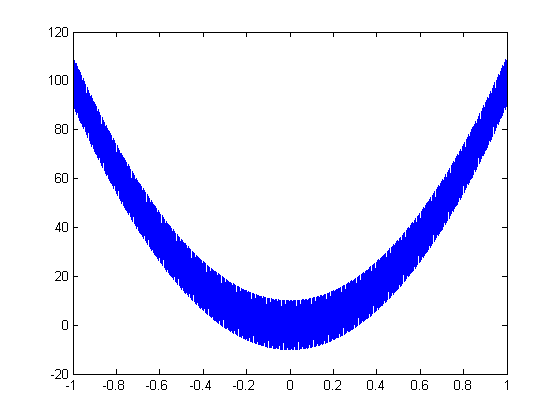
\includegraphics[width=0.5\linewidth]{GSA}
\caption{$y=(10x)^2 + 10 \sin(1000x)$}
\end{figure}
\noindent The global minimum is around -0.00157 where the function is -9.99975. The
value found by the algorithm is 0.02365 and the value of the function is
-9.902866. This result shows us that the method has the possibility of being applied
efficiently for multidimensional problem.



%bibliography
\bibliographystyle{unsrt}
\bibliography{biblio}
%include all the references
\nocite{*}

\end{document}

